\documentclass{article}
\usepackage{amsmath}
\usepackage{graphicx}
\usepackage[margin=1in]{geometry}
\usepackage{booktabs}
\usepackage{array}

\begin{document}
% Header with left date and right name/UIN
\noindent
\begin{minipage}[t]{0.5\textwidth}
    \raggedright
    January 25, 2026
\end{minipage}%
\begin{minipage}[t]{0.5\textwidth}
    \raggedleft
    Joseph DeLeonardis\\
    UIN: 0820000866
\end{minipage}
\vspace{0.5cm}
% Centered title below
\begin{center}
    \textbf{\Large CSCE-636-700}\\
    Deep Learning Homework \#1
\end{center}
\vspace{1cm}

\section*{Problem 1: Changing the Amount of Neurons in Layer 1}

\subsection*{Experimental Setup}

For this experiment, a 2-layer neural network was trained on the MNIST dataset with the following configuration:
\begin{itemize}
    \item \textbf{Architecture:} Dense layer (variable size) → Dense layer (10 neurons, softmax)
    \item \textbf{First layer sizes tested:} 16, 32, 64, 128, 256, 512 neurons
    \item \textbf{Activation function:} ReLU for first layer, softmax for output layer
    \item \textbf{Training parameters:} 5 epochs, batch size of 128, Adam optimizer
    \item \textbf{Loss function:} Sparse categorical crossentropy
\end{itemize}

\subsection*{Results}

The test accuracies for each first layer size were as follows:

\begin{table}[h]
\centering
\begin{tabular}{|c|c|c|}
\hline
\textbf{Number of Neurons} & \textbf{Test Accuracy} & \textbf{Improvement (\%)} \\
\hline
16 & 0.9395 & --- \\
32 & 0.9574 & +1.91 \\
64 & 0.9664 & +0.94 \\
128 & 0.9707 & +0.45 \\
256 & 0.9783 & +0.78 \\
512 & 0.9778 & $-0.05$ \\
\hline
\end{tabular}
\caption{Test accuracy vs. first layer neuron count}
\end{table}

\subsection*{Discussion}

Test accuracy improved considerably with each increase in neuron count until reaching 256 neurons, which achieved optimal performance at 97.83\%. The 512-neuron configuration performed slightly worse at 97.78\%, suggesting the model may be beginning to overfit with excessive network capacity while also requiring additional computational resources.

\begin{figure}[h]
\centering
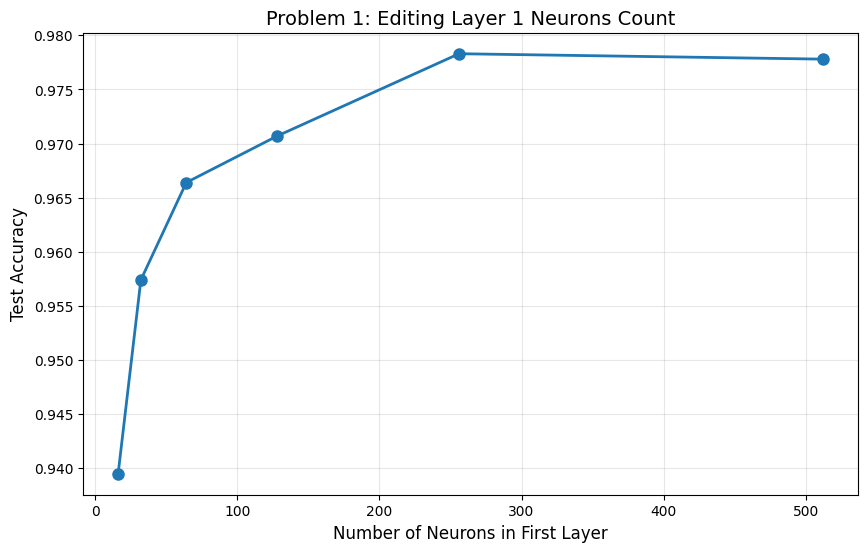
\includegraphics[width=0.8\textwidth]{csce636hw1p1.png}
\caption{Test accuracy vs. first layer neuron count}
\end{figure}

\newpage

\section*{Problem 2: Changing the Amount of Layers}

\subsection*{Experimental Setup}

For this experiment, neural networks with varying depths were trained on the MNIST dataset:
\begin{itemize}
    \item \textbf{Number of layers tested:} 2, 3, 4, 5
    \item \textbf{Architecture design:} Tapering pattern (512 → 256 → 128 → 64)
    \item \textbf{Activation function:} ReLU for hidden layers, softmax for output layer
    \item \textbf{Training parameters:} 5 epochs, batch size of 128, Adam optimizer
    \item \textbf{Loss function:} Sparse categorical crossentropy
\end{itemize}

\subsection*{Layer Architectures}

\begin{table}[h]
\centering
\begin{tabular}{|c|l|}
\hline
\textbf{Number of Layers} & \textbf{Architecture} \\
\hline
2 & 512 → 10 \\
3 & 512 → 256 → 10 \\
4 & 512 → 256 → 128 → 10 \\
5 & 512 → 256 → 128 → 64 → 10 \\
\hline
\end{tabular}
\caption{Network architectures for varying depths}
\end{table}

\subsection*{Results}

The test accuracies for each network depth were as follows:

\begin{table}[h]
\centering
\begin{tabular}{|c|c|c|}
\hline
\textbf{Number of Layers} & \textbf{Test Accuracy} & \textbf{Improvement (\%)} \\
\hline
2 & 0.9778 & --- \\
3 & 0.9785 & +0.07 \\
4 & 0.9767 & $-0.18$ \\
5 & 0.9797 & +0.31 \\
\hline
\end{tabular}
\caption{Test accuracy vs. network depth}
\end{table}

\begin{figure}[h]
\centering
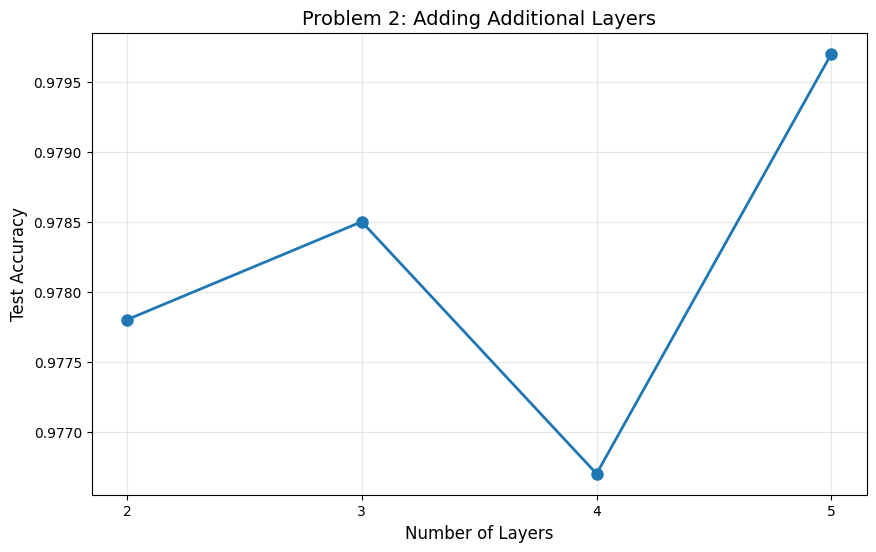
\includegraphics[width=0.8\textwidth]{csce636hw1p2.png}
\caption{Test accuracy vs. network depth}
\end{figure}

\subsection*{Discussion}

The layer architectures were designed using a tapering pattern (512 → 256 → 128 → 64), which is standard practice in neural network design. This approach reflects the principle that early layers extract broad, low-level features requiring more neurons, while deeper layers learn increasingly abstract representations with fewer neurons needed. The results showed modest improvements with added depth, though the 4-layer network was an outlier at 97.67\%. The 5-layer network achieved the best performance at 97.97\%, representing only a 0.19\% improvement over the 2-layer baseline. Given this marginal gain, the performance increase may be attributable to training variance rather than meaningful architectural benefits, suggesting that MNIST is too simple to benefit from deeper layers.

\end{document}
